\chapter{Evaluation and validation}
\label{ch:Eval}

\section{Results}

\subsection{Pretrained on COCO-dataset model}

When applied to images of fine-art photography we can observe that performance of object-detection models is highly variable to some extend because different photographers use different styles to depict their objects in their images.

For example when using an image with a lot of smaller objects (like Andreas Gursky does), performance is rather poor compared to an image with fewer and bigger objects. An example of the pretrained on COCO-dataset Mask R-CNN applied to an Andreas Gursky picture is shown here:

\begin{figure}[H]
	\center{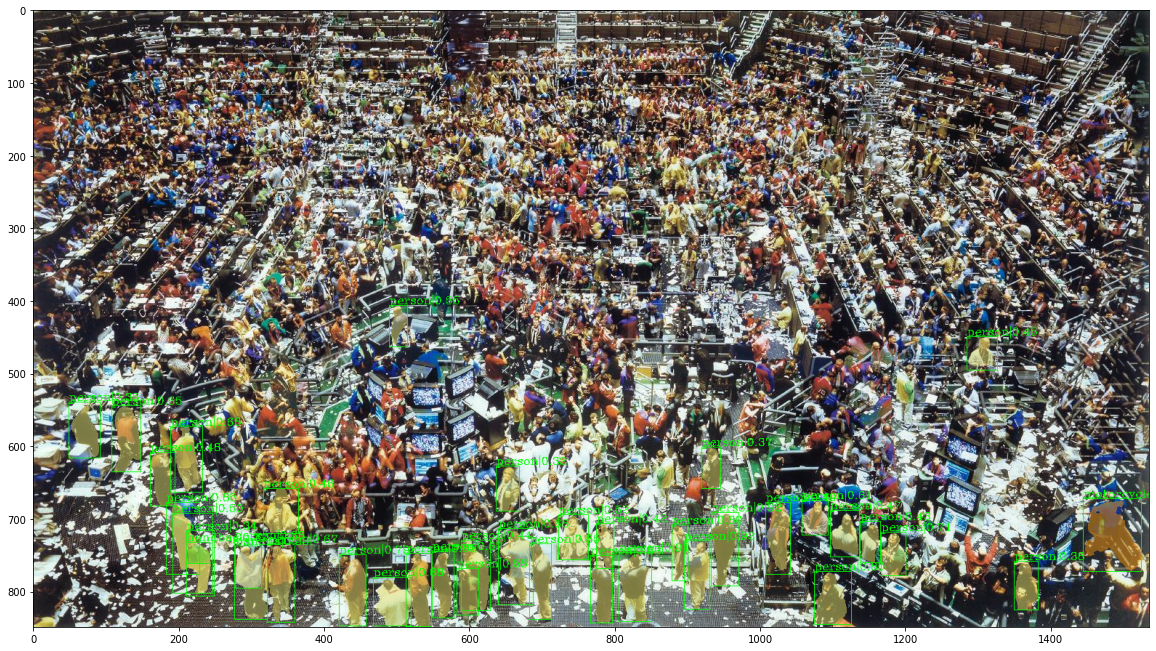
\includegraphics[width=\textwidth]
	{img/gursky-result.png}}
	\caption{\label{fig:fpn} Pretrained model applied on an image from Andreas Gursky}
\end{figure}

As can be seen here, only the largest objects in the foreground (of class "person") got detected. The reason could be because the objects are rather small and photographed from above. However the usage of a FPN should adjust performance when using pictures with small objects depicted. An interesting task would be to train a model especially with pictures from Andreas Gursky to further examine this anomaly.
	
In sum, the performance of the pretrained on COCO-dataset Mask R-CNN model depends on the following criteria: The class of objects depicted in the image (included in COCO-dataset or not), the size of objects in the image, the perspective and angle from which the object was photographed and the degree to which an object is visible and is shown in a natural style.

\subsection{Retrained on "Kunst aufräumen" data model}

As explained in section \ref{refining-the-model} on page \pageref{refining-the-model}, an own model was created by retraining the out-of-the-box R-CNN model via images from "Kunst aufräumen" by Urs Wehrli. The first model, that got retrained was with the car photo. A model could get trained without use of much data augmentation. The reason, as it is my assumption, is that in the car photos, the car objects are just rotated in two different positions: 0° or 180°. Therefore it is not necessary to include random rotations in the training pipeline.

\begin{figure}[H]
\begin{tabular}{cc}
 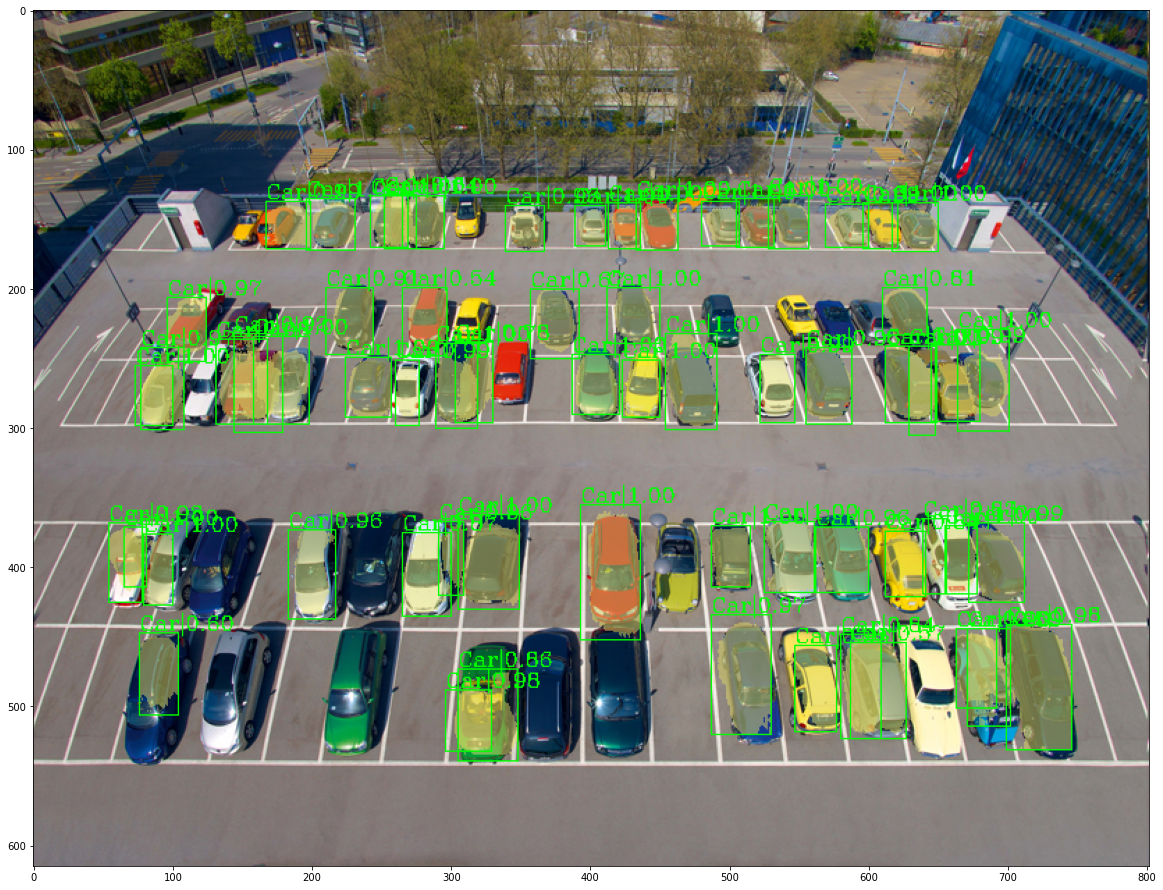
\includegraphics[width=0.5\textwidth]{retrained-only-cars-1500e.png} &   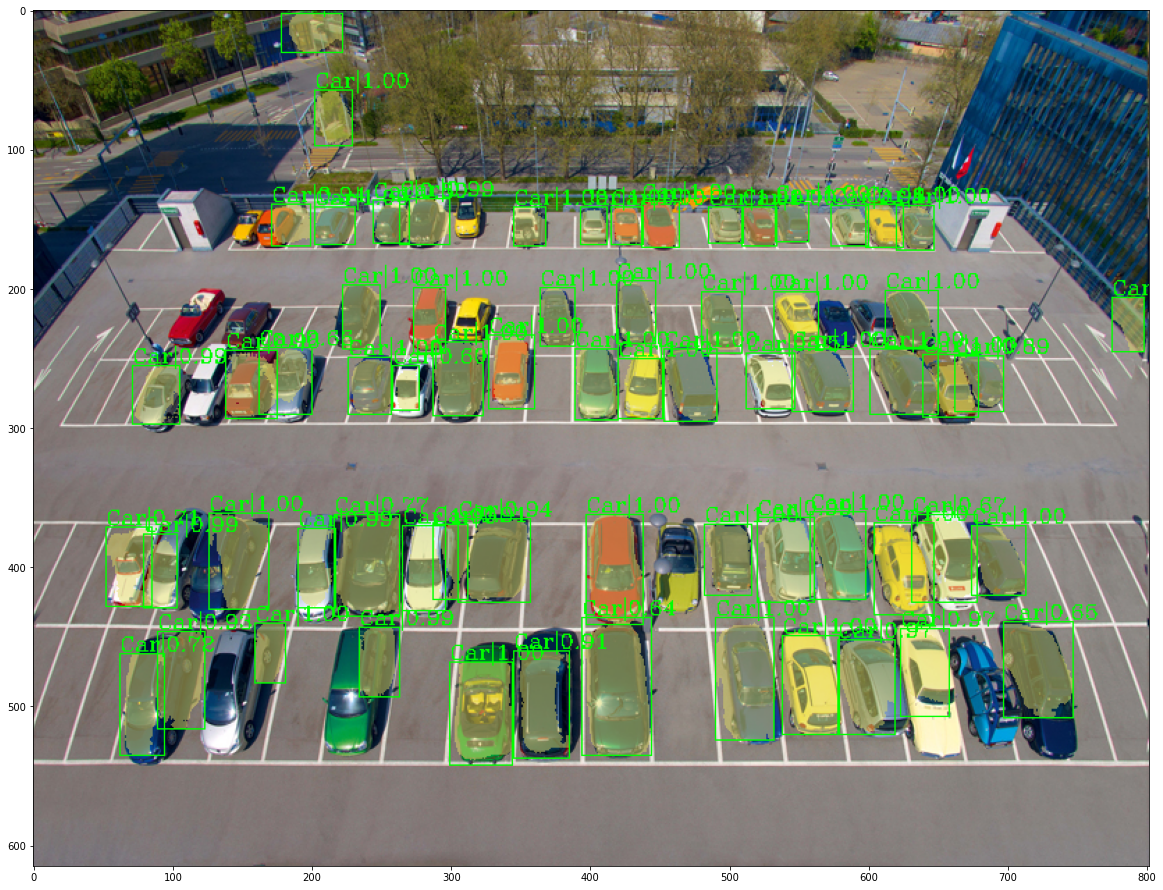
\includegraphics[width=0.5\textwidth]{retrained-only-cars-3000e.png} \\
 (a) 1500 & (b) 3000 \\[6pt]
 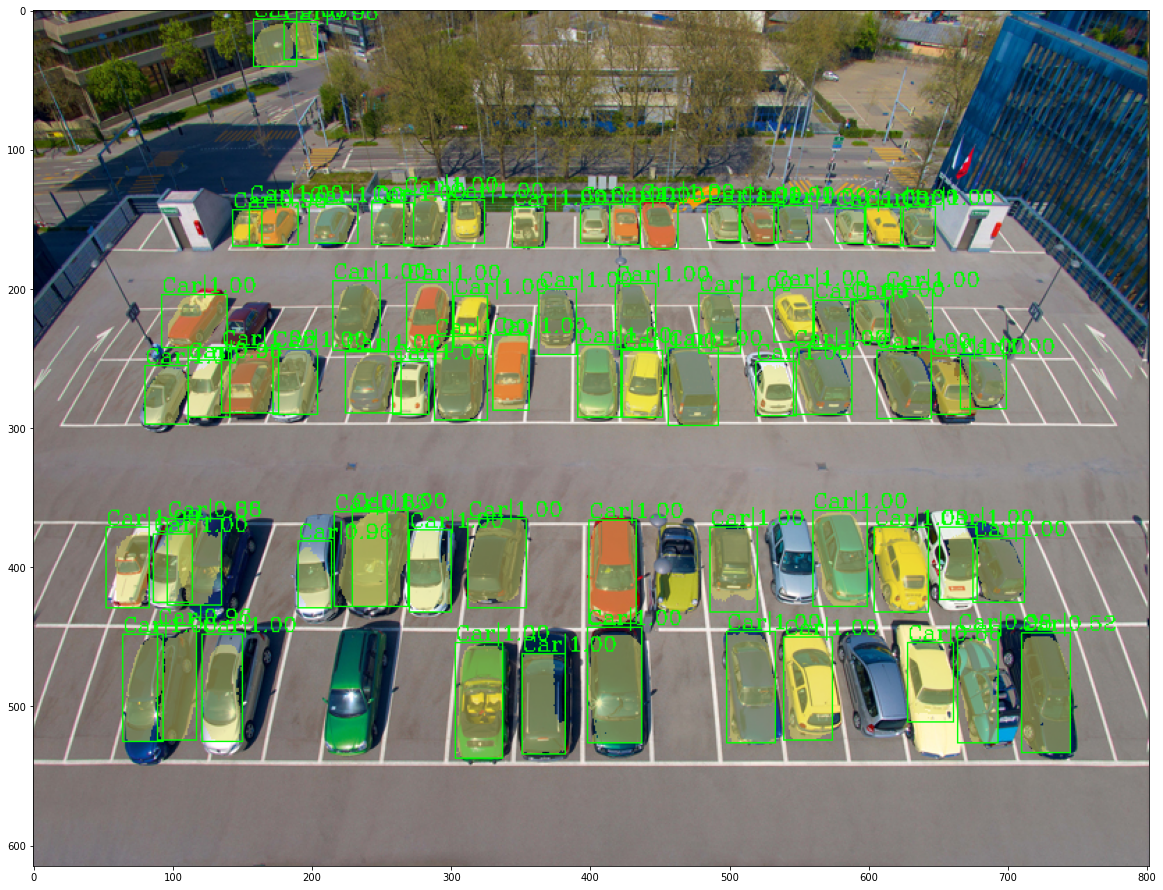
\includegraphics[width=0.5\textwidth]{retrained-only-cars-4500e.png} &   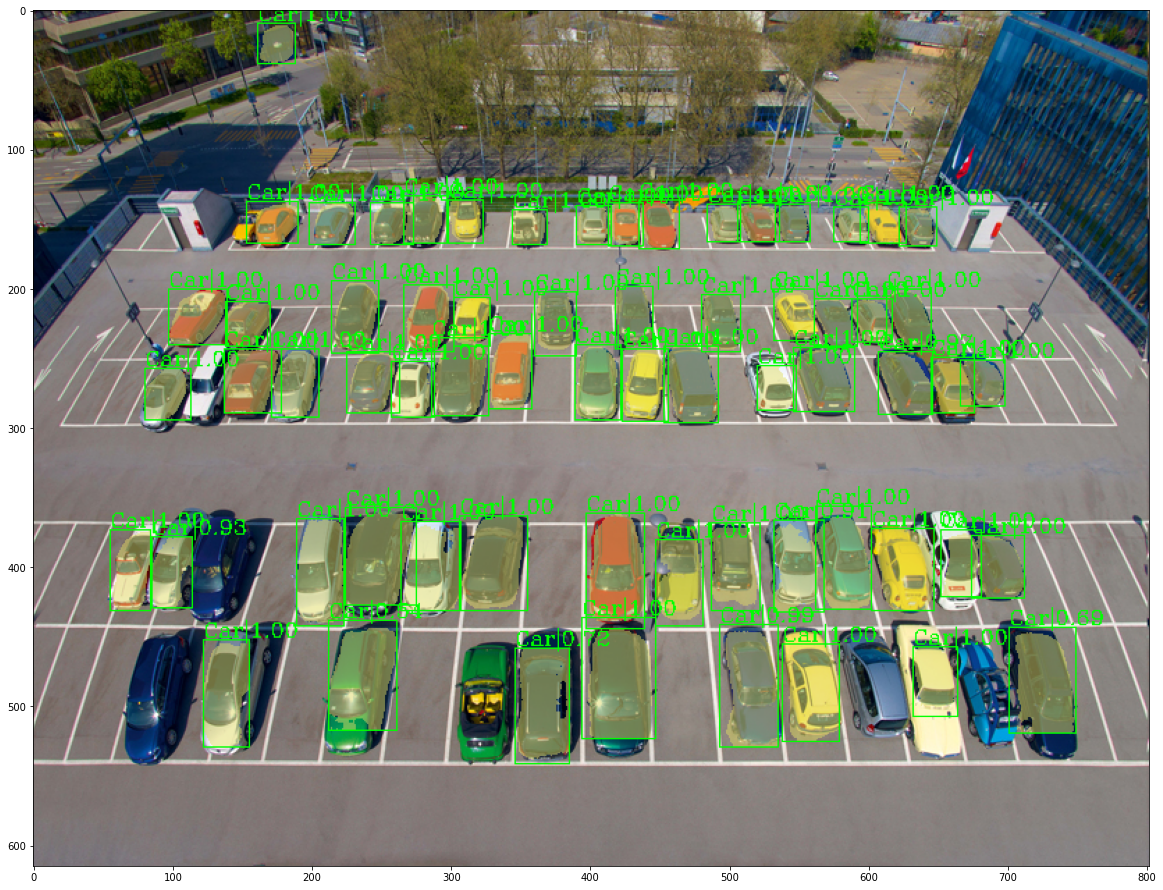
\includegraphics[width=0.5\textwidth]{retrained-only-cars-6000e.png} \\
(c) 4500 & (d) 6000 \\[6pt]
 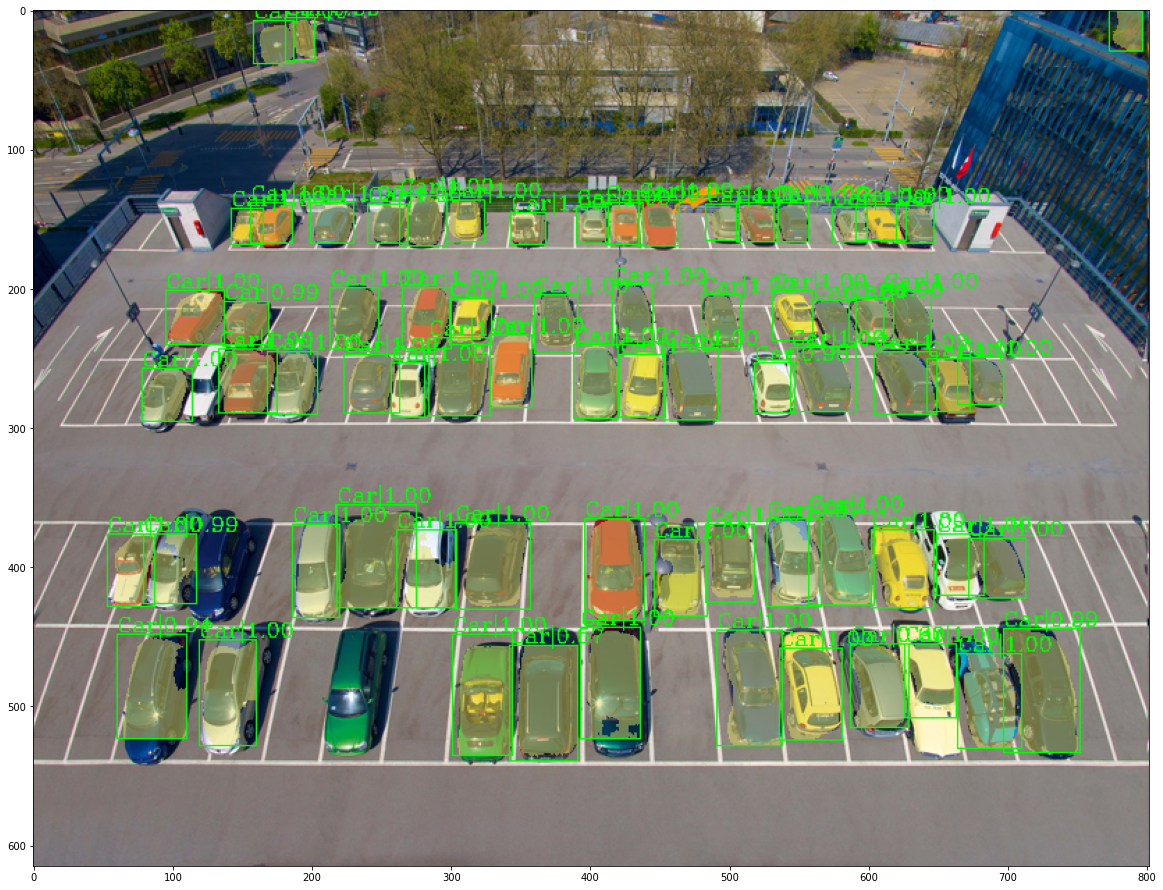
\includegraphics[width=0.5\textwidth]{retrained-only-cars-7500e.png} &   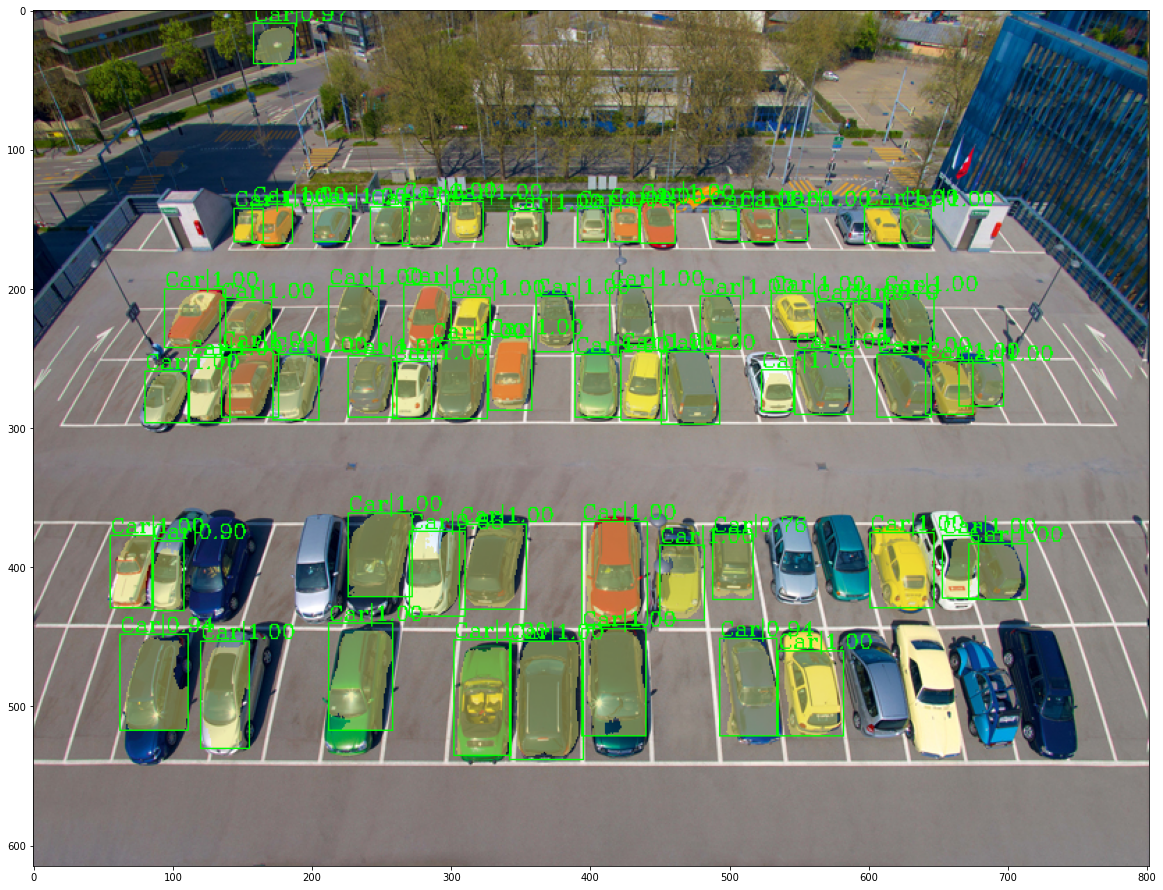
\includegraphics[width=0.5\textwidth]{retrained-only-cars-9000e.png} \\
(e) 7500 & (f) 9000 \\[6pt]
\end{tabular}
\caption{Output of the retrained on "Kunst aufräumen" model, trained with 1500, 3000, 4500, 6000, 7500 and 9000 epochs each.}
\label{fig:epochs-output}
\end{figure}

\section{Reviewing the web application}

The web application is able to fulfil the requirements and is able to solve the given project task. A nice and clean user interface could be designed and developed. However there are some flaws that should be resolved.

\subsection{Weaknesses}

The first thing that got noticed is the very long waiting time until inference is completed. For a large picture, with a lot objects shown, this can be as long as up to 18 seconds or more (using the "Leonard DiCaprio unspoiled" picture from David LaChapelle with a height of 1024px). For a much smaller picture with only few objects, inference time is still about 9 seconds (using the sample COCO-dataset picture from section \ref{why-fine-art} on page \pageref{why-fine-art}. To yield a decent user experience, calculation time should not exceed two seconds. By switching to a GPU-powered infrastructure, this lack of performance could possibly be solved very easily.

\subsection{Known bugs}

\section{Comparison with given requirements}

The following tasks were successfully accomplished: A dataset, containing of 42 images from four different artist, has been gathered. Different object detection models and frameworks have been tested out on this dataset on Google Colab. The most promising model has been chosen to implement in a web application. The web application has been developed and deployed on the EnterpriseLab successfully. An own model has been created by refining the pretrained on COCO-dataset model with new data from "Kunst aufräumen".

Unfortunately there was no time left over to develop an own metric to examine and compare different models when applied to pictures of artistic photography.

\section{Evaluation of technical tools}

Retrospectively, the used toolchain emerged to be highly effective. Google Colab is a very powerful infrastracture, especially when one does not possess an own Nvidia GPU. To share and comment whole notebooks or single cells was a big plus.

MMDetection turned out to be a fast, modular and powerful framework for computer vision projects. Very helpful was the ability to save checkpoints and to resume training at a later point of time. MMDetection received a lot of traction in the last years and is in a steady change, version 2.0.0 just got released in April 2020.

Plotly-Dash was a joy to work with, as it lets the developer turn a Python program into a full-fledged web application very quickly with minimal overhead. As it is built upon JavaScript technologies (React), it is highly customizable too. There exists a lively community that is eager to help.

Unluckily, to this day, most frameworks do not support operating on CPU in inference mode (however this was fixed in MMDetection 2.0.0 in April 2020). To accomplish this, an indirection via SMD, as explained in \ref{inference-cpu} on page \pageref{inference-cpu} had to be taken. Running the inference on CPU has one major drawback: It slows down computation time badly. To serve the best performance and user experience, a GPU-powered server infrastructure should be taken into consideration.

\section{Evaluation of used method}

The used approach, to proceed to retraining, after the whole toolchain got finished, turned out to be the right decision. However not all milestones could be reached in the agreed point of time, as can be seen in the next section.

\subsection{Evaluation of project management and project procedure}

Due to several problems and bugs, the achievement of certain milestones was delayed for some time:

\begin{table}[H]
\begin{tabular}{@{}lll@{}}
\toprule
Milestone & Agreed date & Actual date \\ \midrule
Test pretrained models on Google Colab with new data & 24th March 2020 & 24th March 2020 \\
Build web application prototype & 28th April 2020 & 5th May 2020 \\
Finetune model with fine art photography data & 12th May 2020 & 31th May 2020 \\
Test finetuned model on new data & 19 May 2020 & 31th May 2020 \\
Finish web application with new model & 2nd June 2020 & 3rd June 2020
\end{tabular}
\caption{Agreed and actual dates of all milestones}
\label{tab:milestones}
\end{table}
	
\subsection{Project difficulties}

